\PassOptionsToPackage{unicode}{hyperref}
\documentclass[aspectratio=1610, professionalfonts, 9pt]{beamer}

\usefonttheme[onlymath]{serif}
\usetheme[showtotalframes]{tudo}



\ifluatex
  \usepackage{polyglossia}
  \setmainlanguage{german}
\else
  \ifxetex
    \usepackage{polyglossia}
    \setmainlanguage{german}
  \else
    \usepackage[german]{babel}
  \fi
\fi


% Mathematik
\usepackage{amsmath}
\usepackage{amssymb}
\usepackage{mathtools}
\usepackage{cancel}

\usepackage{hyperref}
\usepackage{bookmark}

%%%%%%%%%%%%%%%%%%%%%%%%%%%%%%%%%%%%%%%%%%%%%%%%%%%%%%%%%%%%%%%%%%%%%%%%%%%%%%%%
%%%%%-------------Hier Titel/Autor/Grafik/Lehrstuhl eintragen--------------%%%%%
%%%%%%%%%%%%%%%%%%%%%%%%%%%%%%%%%%%%%%%%%%%%%%%%%%%%%%%%%%%%%%%%%%%%%%%%%%%%%%%%

%Titel:
\title{Theoretische Untersuchung von Formfaktoren in $\overline{B} \to D l \overline{\nu}_l$}
%Autor
\author[J.~Alameddine]{Jean-Marco Alameddine}
%Lehrstuhl/Fakultät
\institute[Lehrstuhl für Theoretische Physik IV]{Lehrstuhl für Theoretische Physik IV}
%Titelgrafik
%\titlegraphic{\includegraphics[width=0.7\textwidth]{images/tudo-title-2.jpg}}
\date[27.09.2017]{27. September 2017}

\setbeamertemplate{navigation symbols}{}
\setbeamertemplate{section in toc}[circle]

\begin{document}

\maketitle

\begin{frame}{Inhaltsverzeichnis}
  \tableofcontents[]
\end{frame}

\section{Einleitung}


\begin{frame}{Inhaltsverzeichnis}
  \tableofcontents[currentsection,currentsubsection,
      hideothersubsections,
      sectionstyle=show/shaded,
  ]\end{frame}

\begin{frame}
  \begin{minipage}{8cm}
  \begin{itemize}
    \item<1-> Untersuchung des Standardmodelles der Teilchenphysik
    \item<3-> Betrachteter Zerfall: $\overline{B} \to D l \overline{\nu}_l$
    \item<5-> Untersuchte Observable: $R(D)$
    \item[→]<6-> Diskrepanz zwischen theoretischen und experimentellen Ergebnissen
  \end{itemize}
  \end{minipage}%
  \begin{minipage}{7cm}
  \begin{overprint}
    \onslide<2>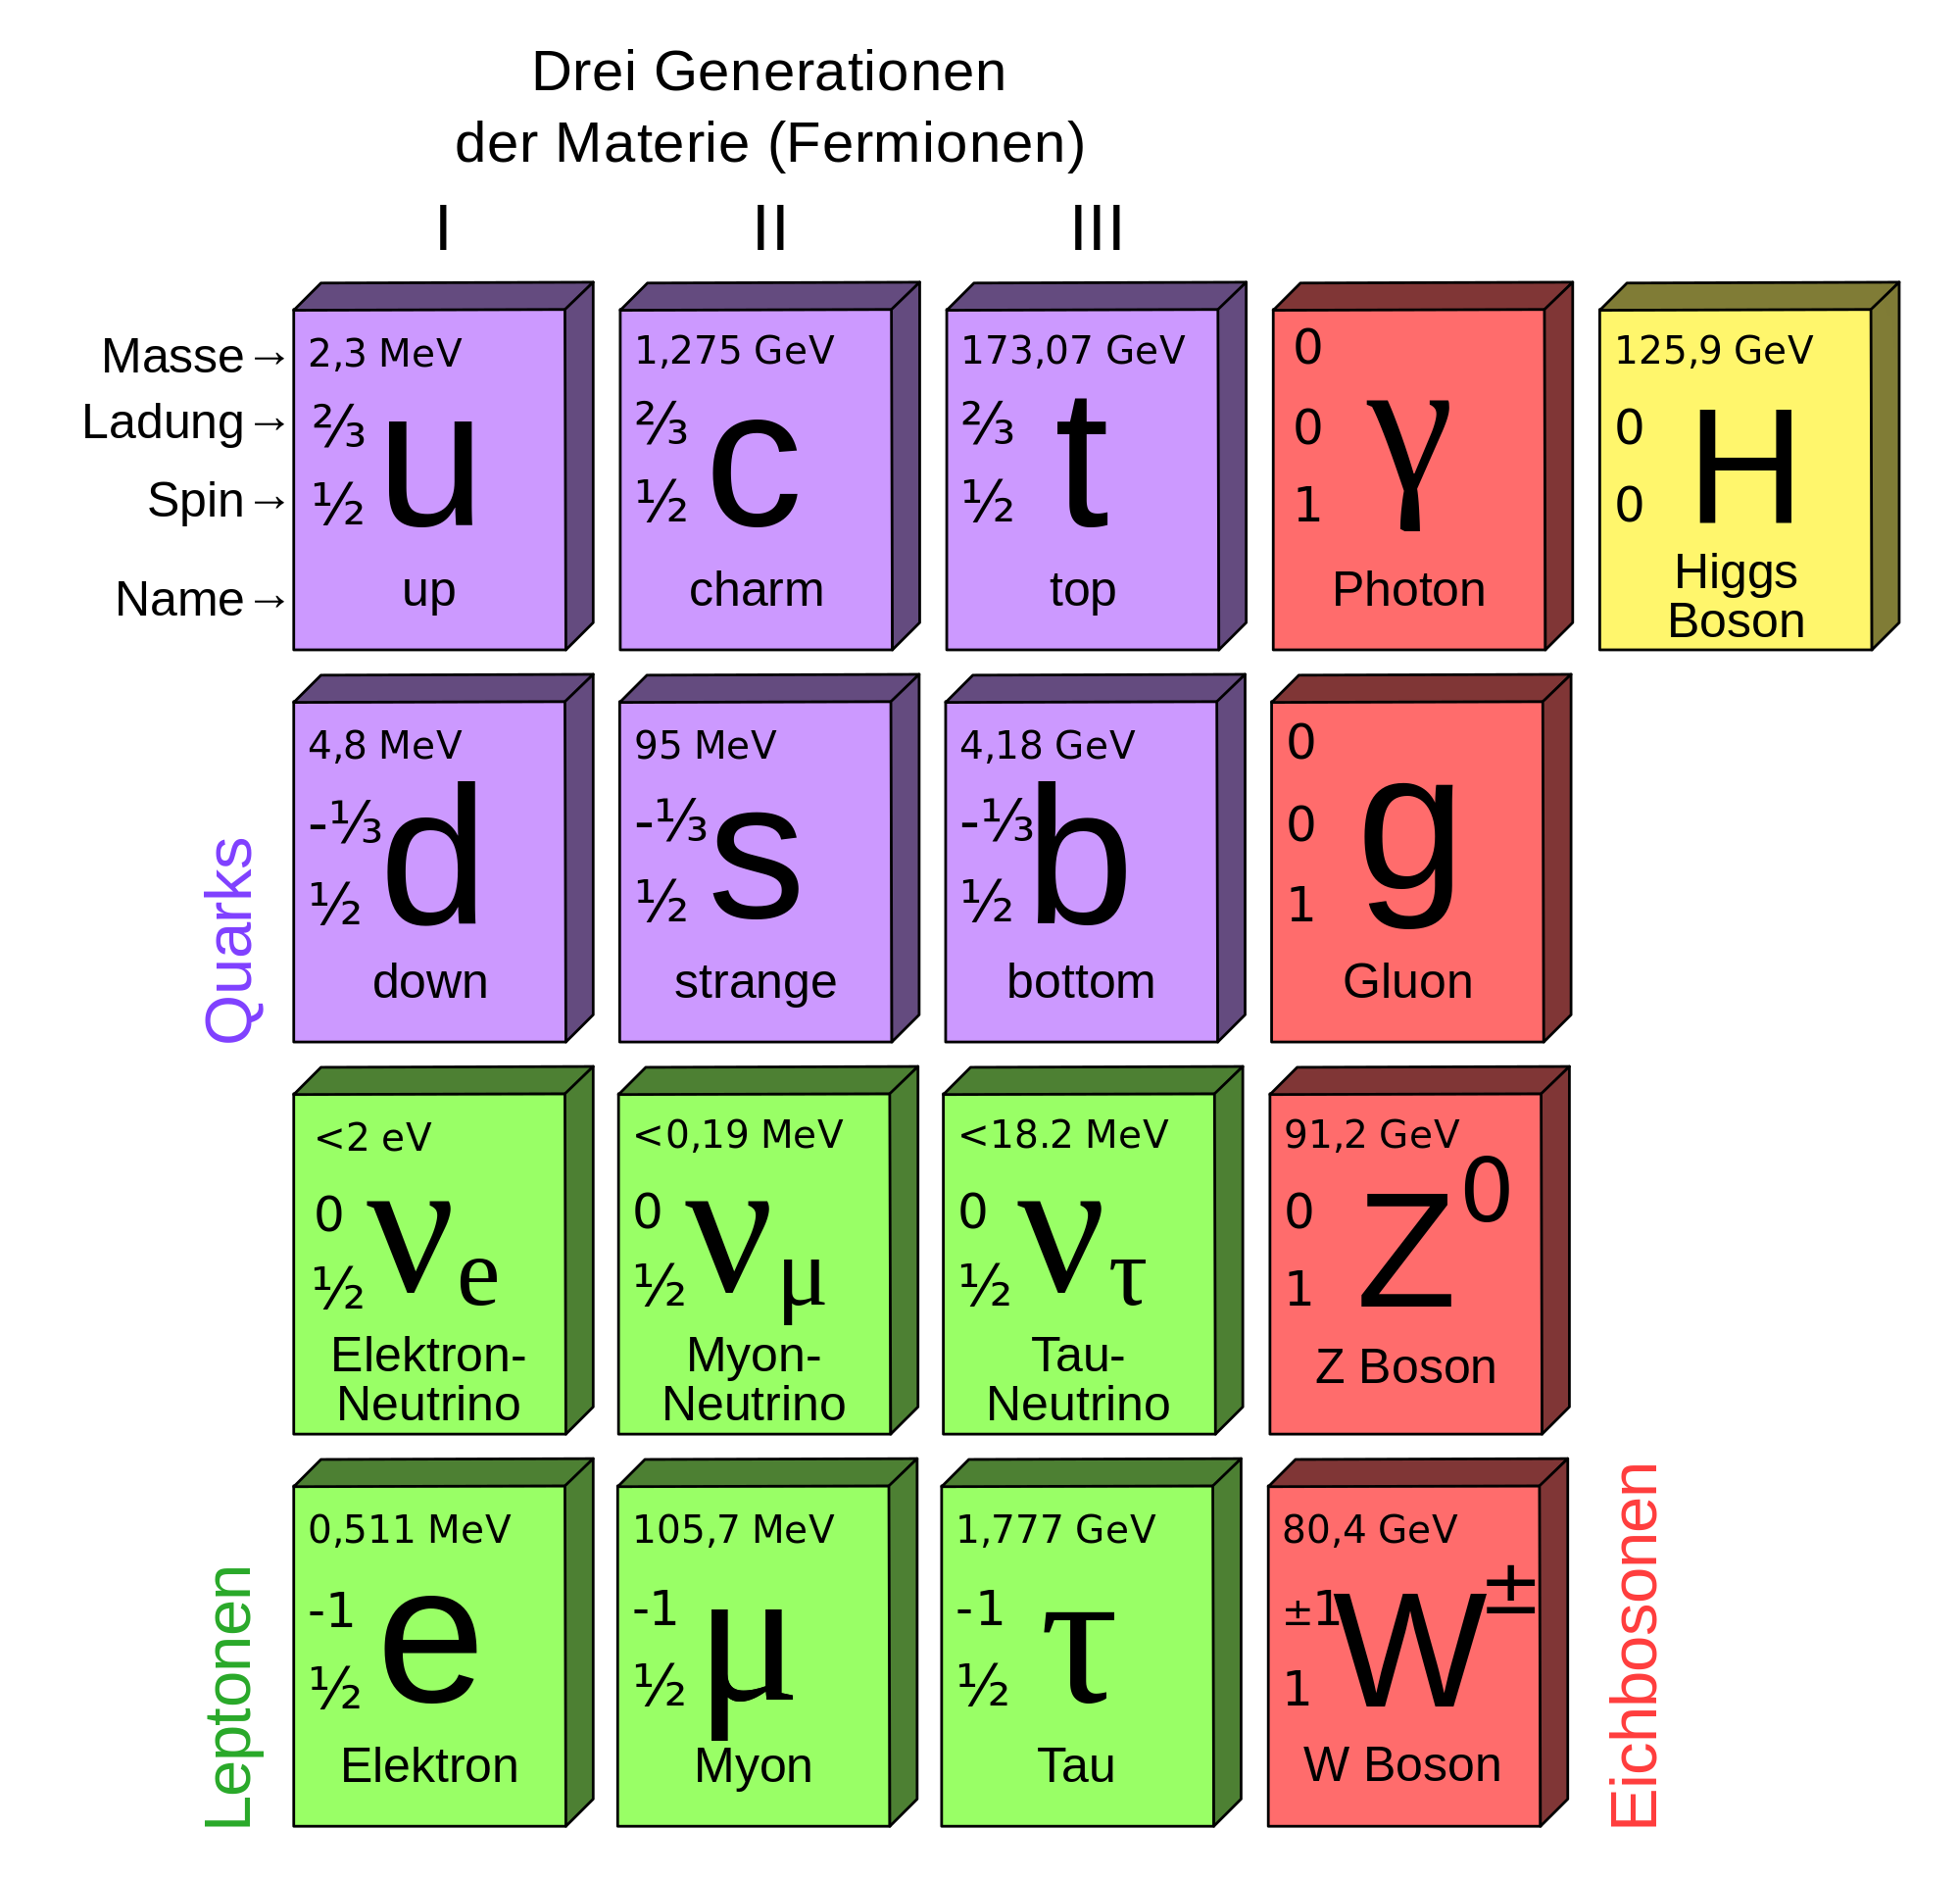
\includegraphics[height=7cm, width=6.7095cm]{Standard_Model_of_Elementary_Particles-de_colorlfull.png}
    \onslide<3>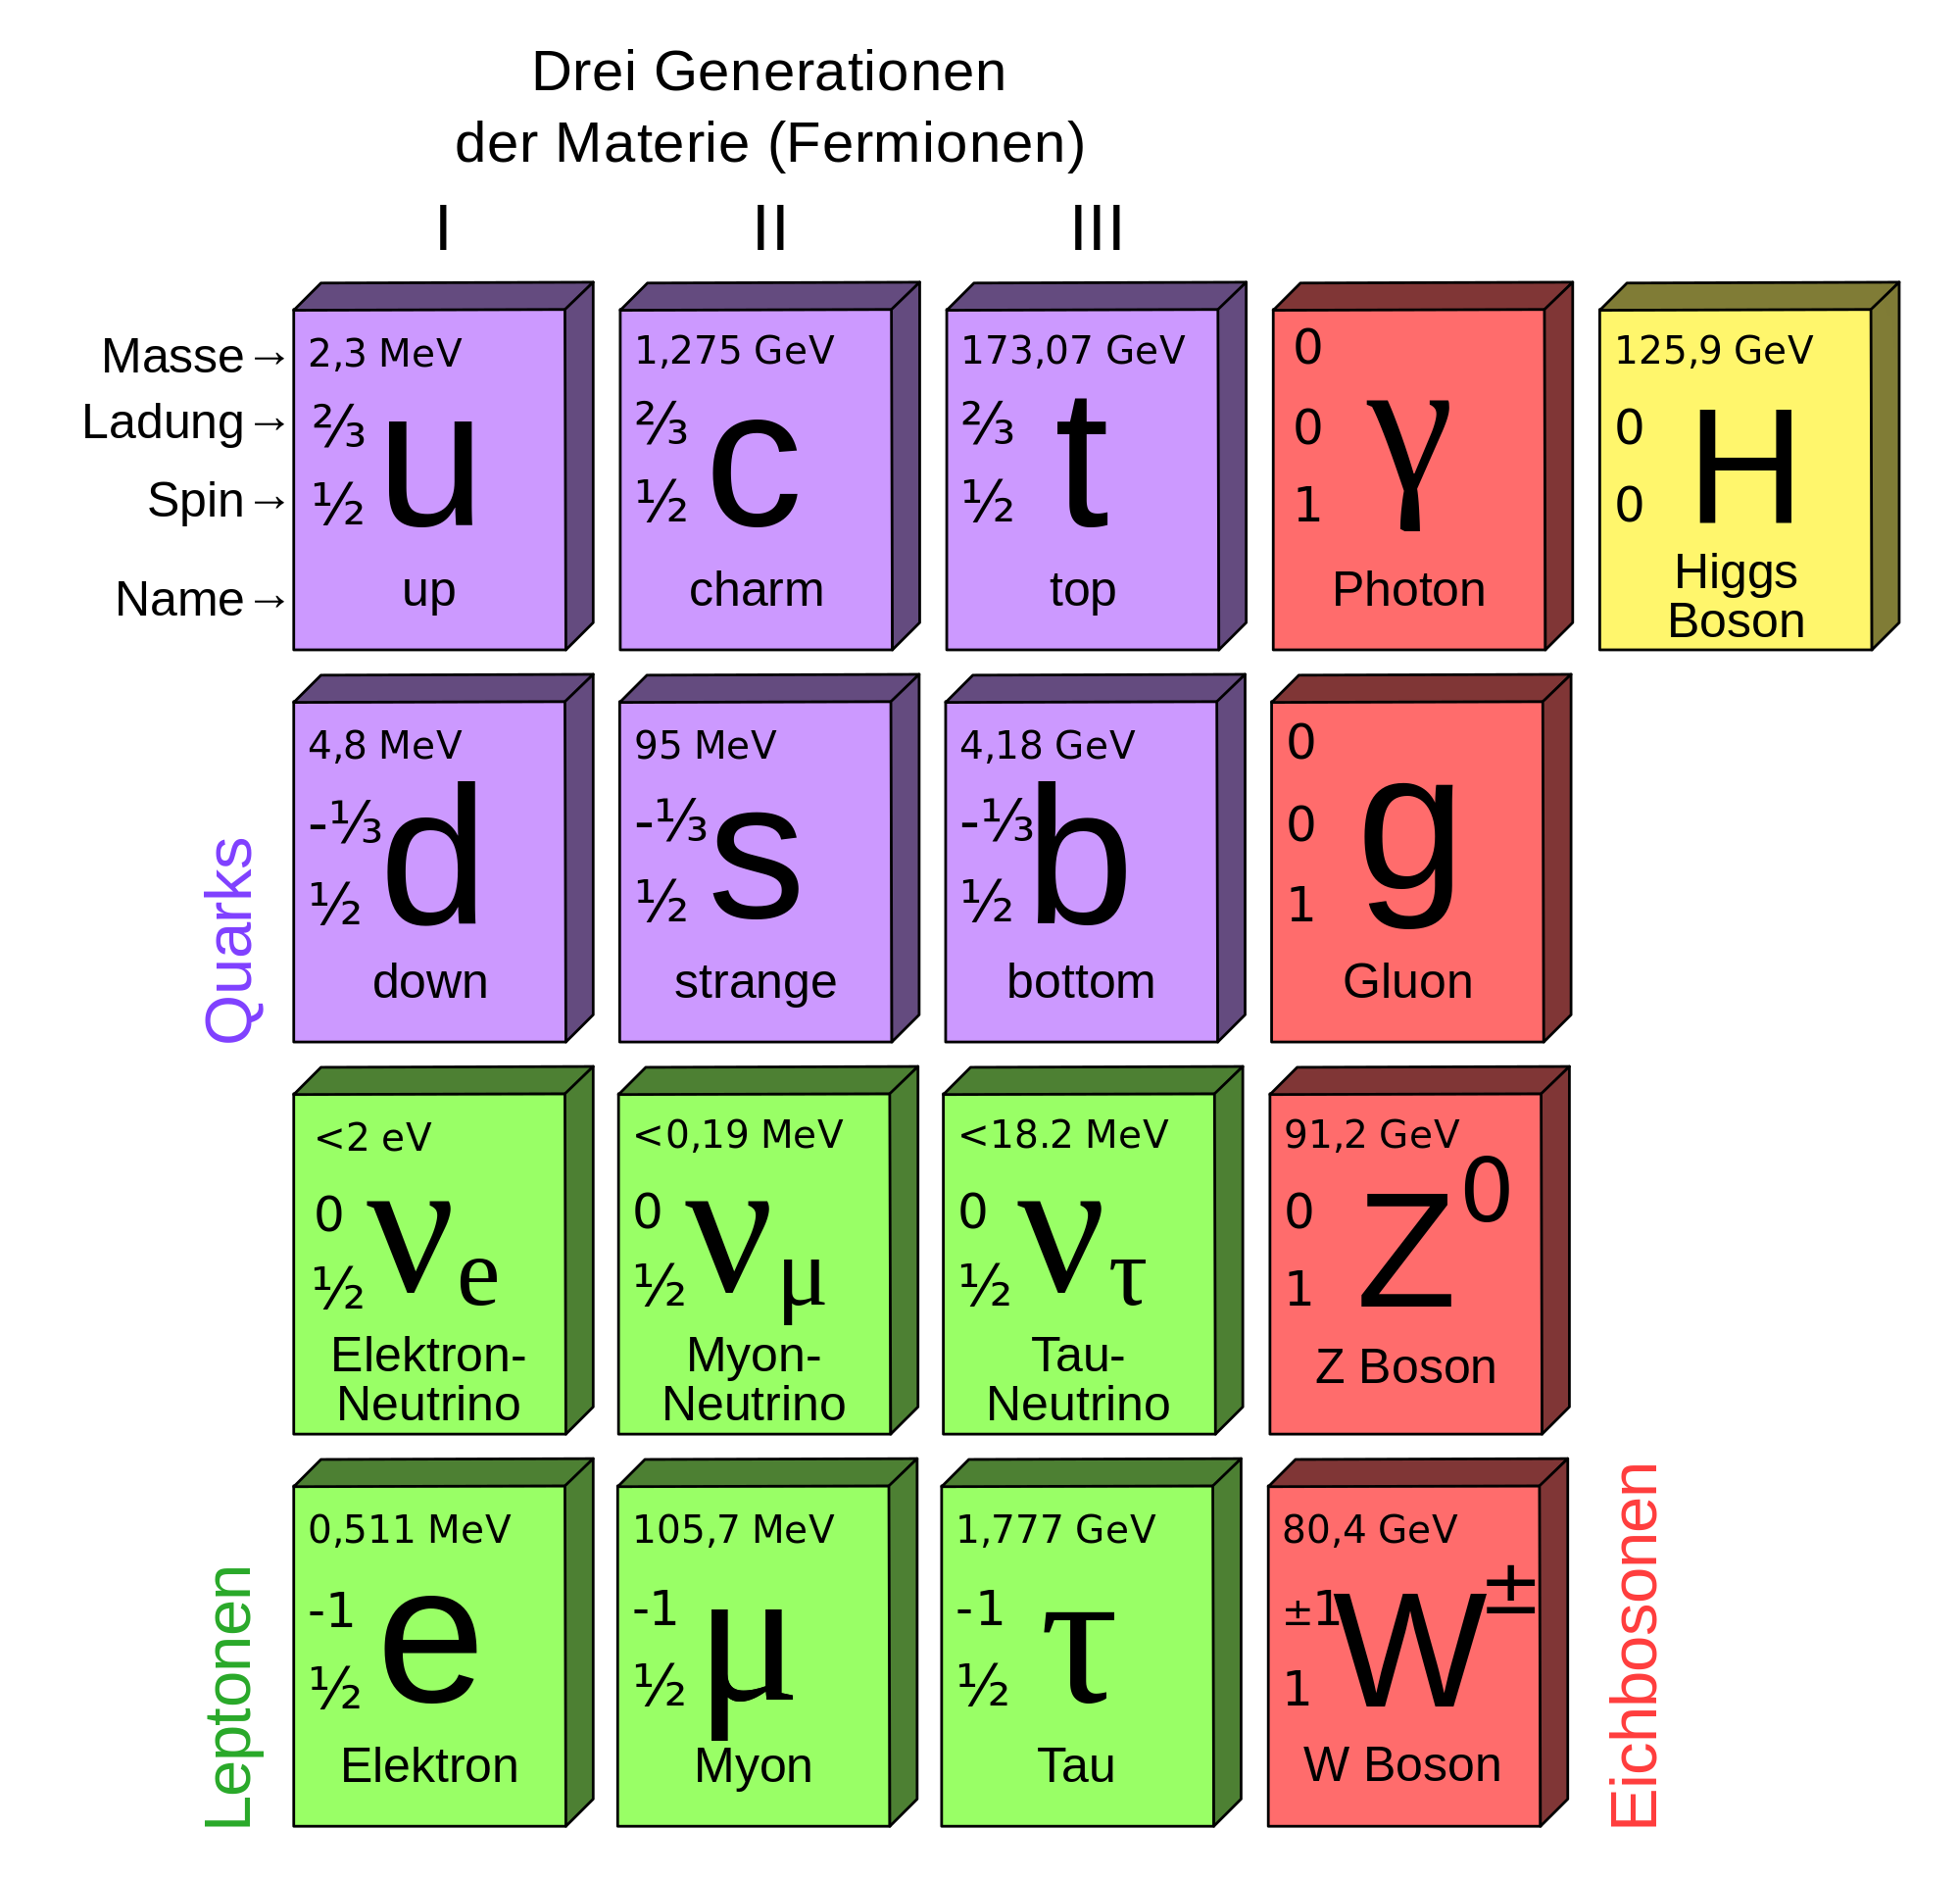
\includegraphics[height=7cm, width=6.7095cm]{Standard_Model_of_Elementary_Particles-de_colorlfull.png}
    \onslide<4->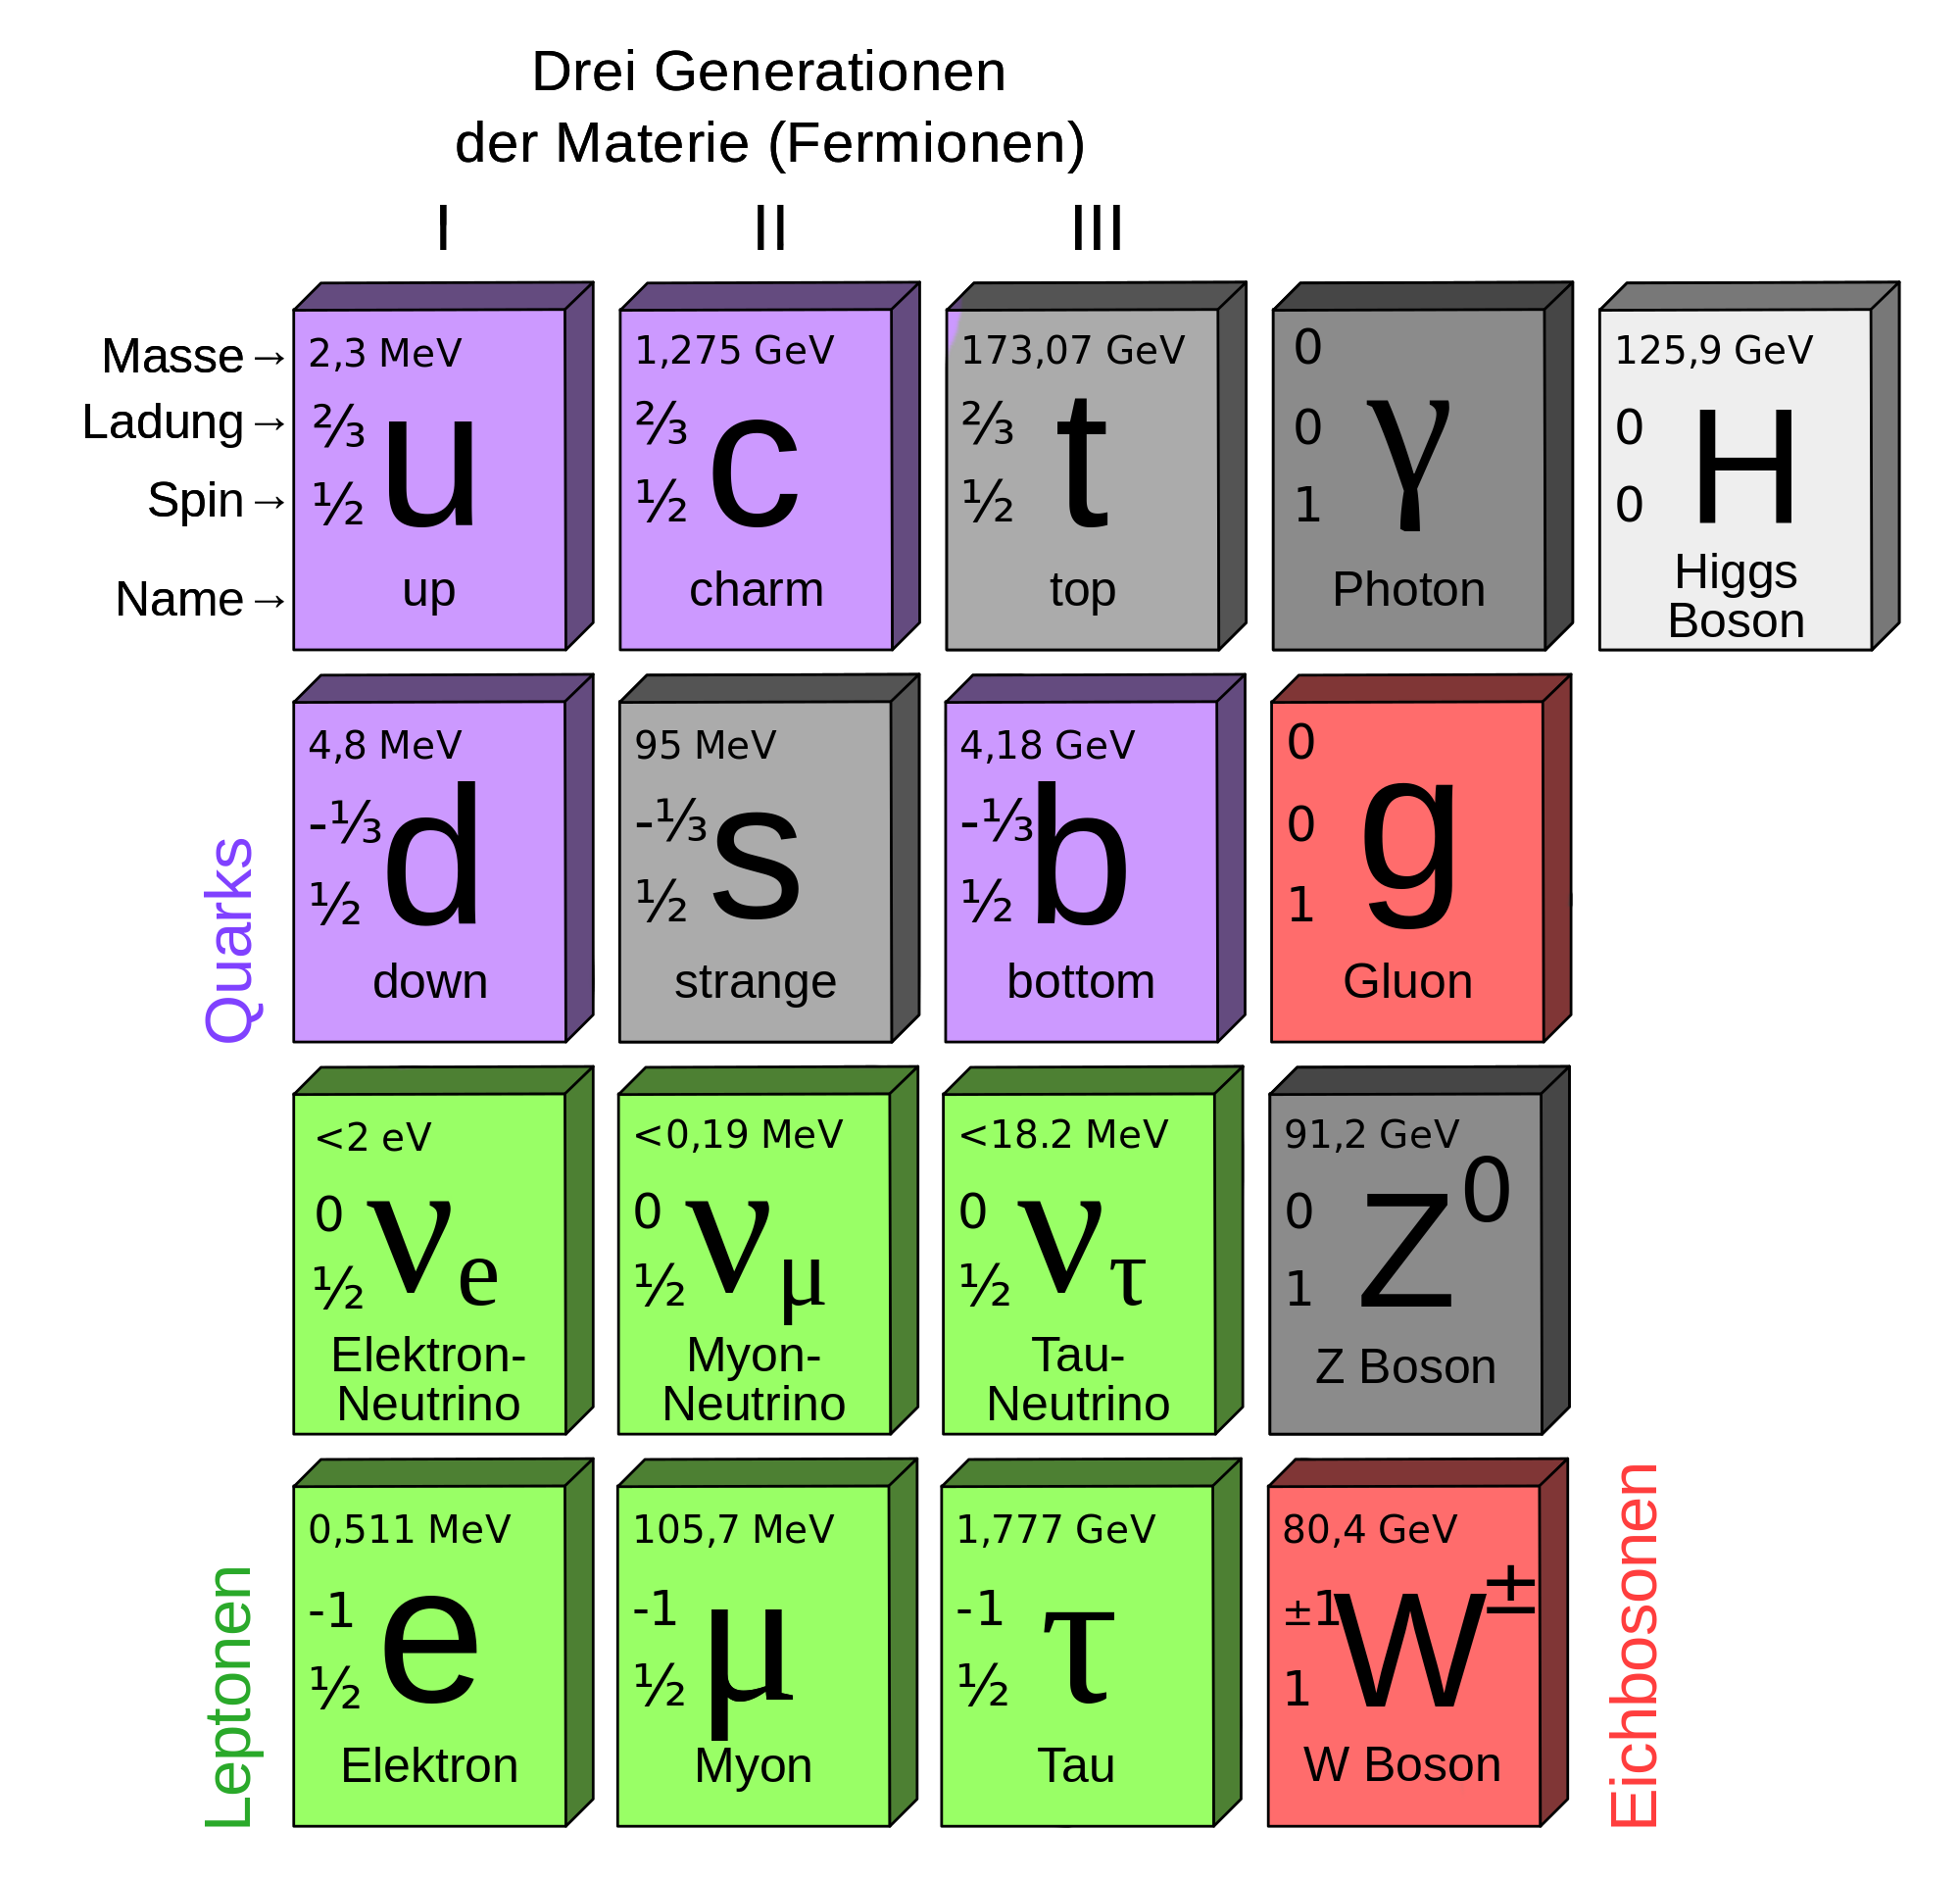
\includegraphics[height=7cm, width=6.7095cm]{Standard_Model_of_Elementary_Particles-de_colorless.png}
  \end{overprint}
  \end{minipage}
\end{frame}

\section{Theorie}

\begin{frame}{Inhaltsverzeichnis}
  \tableofcontents[currentsection,currentsubsection,
      hideothersubsections,
      sectionstyle=show/shaded,
  ]\end{frame}

\begin{frame}
    Hier erzähle ich Theorie.
\end{frame}

\section{Fit}

\begin{frame}{Inhaltsverzeichnis}
  \tableofcontents[currentsection,currentsubsection,
      hideothersubsections,
      sectionstyle=show/shaded,
  ]\end{frame}

\begin{frame}
    Hier fitte ich.
\end{frame}

\begin{frame}
    Weitere Fits.
\end{frame}

\section{Zusammenfassung}

\begin{frame}{Inhaltsverzeichnis}
  \tableofcontents[currentsection,currentsubsection,
      hideothersubsections,
      sectionstyle=show/shaded,
  ]\end{frame}

\begin{frame}
    Hier fasse ich zusammen.
\end{frame}

\section{Diskussion}

\begin{frame}{Inhaltsverzeichnis}
  \tableofcontents[currentsection,currentsubsection,
      hideothersubsections,
      sectionstyle=show/shaded,
  ]\end{frame}

\end{document}
